ระบบระบุตัวตนของบุคคล\textsuperscript{\cite{luo2019alignedreid++}} คือการระบุตัวตนของบุคคลภายในวิดีโอหรือระหว่างรูป 2 รูป สามารถนำมาประยุกต์ใช้ในด้านของการรักษาความปลอดภัย 
การตามหาบุคคล หรือการตรวจสอบการกระทำของบุคคลนั้นในวิดีโอได้ ซึ่งการระบุตัวตนของบุคคลนั้นเป็นปัญหาที่ท้าทาย 
เนื่องจากคุณลักษณะทั่วไปของบุคคลในรูปไม่เพียงพอต่อการระบุบุคคลภายในรูปว่าเป็นบุคคลคนเดียวกันได้ 
ซึ่งวิธีการที่ใช้สำหรับการระบุตัวตนของบุคคลเรียกว่า Dynamically Matching Local Information (DMLI) ที่สามารถจัดแนวรายละเอียดข้อมูลของรูป และเพิ่มประสิทธิภาพให้สูงขึ้น

\begin{figure}[!ht]
	\centering
	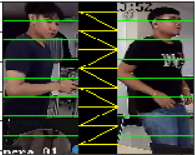
\includegraphics[width=0.3\textwidth]{chapter2/images/alignedreid.png}
		\caption{การแบ่งรูปออกเป็น 8 ส่วนของระบบระบุตัวตนของบุคคล}
    	\label{fig:alignedreid}
\end{figure}

การทำงานของระบบระบุตัวตนของบุคคลจะเริ่มจากการแบ่งรูปออกเป็น 8 ส่วนและนำคุณลักษณะของรูปมาผ่านกระบวนการ normalization เพื่อลดความซ้ำซ้อนของข้อมูล 
แล้วนำมาเปรียบเทียบความแตกต่างของคุณลักษณะของรูป หลังจากนั้นหาค่าเฉลี่ยของความแตกต่างออกมา โดยค่าที่ได้ออกมาจะเรียกว่า original distance ถ้าค่าที่ออกมาใกล้เคียงกับ 0 จะหมายถึงบุคคลในรูปทั้งสองเป็นบุคคลเดียวกัน  และมีการตั้งค่าเกณฑ์สำหรับ original distance เพื่อใช้สำหรับในการระบุบุคคลในรูปเป็นบุคคลเดียวกัน


โดยชุดข้อมูลที่นำมาใช้สำหรับการทำโมเดลปัญญาประดิษฐ์ได้แก่
\begin{enumerate}
	\item {Market1501 เป็นชุดข้อมูลที่เก็บข้อมูลภาพของบุคคลโดยใช้กล้องจำนวน 6 ตัว ถ่ายภาพบุคคลที่ด้านหน้าของซุปเปอร์มาร์เก็ตในมหาวิทยาลัย Tsinghua}
	\item{DukeMTMCReID เป็นชุดข้อมูลที่เก็บข้อมูลภาพของบุคคลโดยใช้กล้องจำนวน 8 ตัว ถ่ายภาพบุคคลที่วิทยาเขตของมหาวิทยาลัย Duke ซึ่งมีการเก็บภาพมากถึง 2 ล้านภาพของนักศึกษา 2 พันคน }
	\item{CUHK-03 เป็นชุดข้อมูลที่เก็บภาพของบุคคลที่มหาวิทยาลัยจีนที่ฮ่องกง}
	\item{MSMT17 เป็นชุดข้อมูลที่เก็บข้อมูลภาพของบุคคลโดยใช้กล้องจำนวน 15 ตัว โดยที่กล้องแต่ละตัวจะไม่ได้ตั้งอยู่สถานที่เดียวกัน และเก็บข้อมูลที่ในวันที่มีสภาพอากาศต่างกัน}
\end{enumerate}

โดยทุกชุดข้อมูลจะใช้ ResNet50 ในการสร้างโมเดลปัญญาประดิษฐ์ สำหรับการต่อมาการทดสอบโมเดลปัญญาประดิษฐ์ด้วยวิธีการ Global+DMLI คือวิธีการนำคุณลักษณะทั่วไปของภาพนำไปจัดแนวรายละเอียดของข้อมูล และนำไปเข้าโมเดลปัญญาประดิษฐ์เพื่อคำนวณหาค่า rank1 และ mAP โดยที่ค่า rank1 หมายถึงค่าเปอร์เซ็นต์ความมั่นใจสูงสุดของโมเดลปัญญาประดิษฐ์ที่ทำนายออกมาถูกต้อง และค่า mAP คือการหาค่าเฉลี่ยความแม่นยำในแต่ละหมวดหมู่ ซึ่งสามารถดูค่า rank1 และ mAP ของโมเดลปัญญาประดิษฐ์สำหรับการทำระบุตัวตนของบุคคลได้ที่การทดสอบประสิทธิภาพการทำงานของโมเดลปัญญาประดิษฐ์สำหรับการระบุตัวตนของมนุษย์